\documentclass[letterpaper]{article}
\usepackage{natbib,alifexi}
\usepackage{float}
\usepackage[labelfont=bf]{caption}

\title{Project Computational Game Theory\\Evolution of All-Or-None Strategies in Repeated Public Goods Dilemmas}
\author{Ruben Vereecken, Yoni Pervolarakis \and Laurens Hernalsteen \\
\mbox{}\\Vrije Universiteit Brussel \\Pleinlaan 2, \\B-1050 Brussels, BELGIUM\\
{\texttt{\{rvereeck,ypervola,lhernals\}@vub.ac.be}}}


\begin{document}
\maketitle

\begin{abstract}
Engaging in repeated group interactions such as \textit{Public Good Games}  (\textbf{PGG}), groups of individuals may contribute to a common pool and subsequently share their resources. In this paper we will recreate the research and results from the paper  \textit{Evolution of All-Or-None Strategies in Repeated Public Goods Dilemmas}  \citep{project}. Studying evolutionary dynamics, where individuals behave on what they observed in the previous round, the simple \textit{All-Or-None} \textbf{(AON)} strategy  \textbf{will emerge} \footnote{Or not? Wait for results.}. AON consists of cooperating only after an unanimous group choice. We prove the \textbf{robustness of this strategy} \footnote{Will we?}by using different group sizes and error rates
\textit{\textbf{Short summary of results....}}


\end{abstract}

\section{Introduction}
When studying \textit{Public Good Games}  (\textbf{PGG}), such as \textit{N-person Prisoner's Dilemma}  (\textbf{NPD}), social dilemmas arise where self-serving behavior is worse than collective behavior \citep{kollock1998social}. These problems can be found in economics as well in biology.
Without additional mechanisms such as risk of future loss \citep{santos2011risk}, institutions who deal with free-riders who choose not to contribute \citep{vasconcelos2013bottom,sigmund2010social}, thresholds that must be surpassed before collecting action can be successful \citep{pacheco2011evolutionary}, a network of interactions or social diversity \citep{wang2013interdependent,santos2008social}, punishment \citep{fehr2002altruistic,brandt2006punishing} or voluntary participation \citep{hauert2002volunteering} there is a possibility that populations will fall into a tragedy of the commons \citep{hardin1968tragedy}.
Collective action problems often involve repeated actions between individuals of the same group \citep{boyd1988evolution}. Real life examples can be found in world leaders trying to cooperate in changing the climate problems \citep{milinski2008collective,barrett2012climate}, the monetary crisis \citep{jacquet2001economic} and even in anarchies \citep{axelrod1985achieving}. This leads to the question whether direct reciprocity can escape the tragedy of the commons. If we subdivide this question, it is difficult to find to whom one should reciprocate in repeated N-player interactions. Direct reciprocity has been generalized for \textbf{PGG} where individuals of group size N only cooperate if there are at least M $(0<=M<=N)$ cooperators in the previous round \citep{van2012emergence,kurokawa2009emergence}. Such generalized reciprocators provide a generalization of the \textit{Tit For Tat}  (\textbf{TFT}) strategy, but they constitute a small set of all individual strategies.
In this research exploration of different strategies will be researched, where individuals may adopt a different strategy when playing \textbf{PGG} on the condition that their actions are based on the behavior of the group in the previous round.
\textit{\textbf{more??}}

\section{Methods}
Let us consider a finite and will-mixed population $Z$, with only cooperators and defectors, who randomly form groups of size $N$ and play the repeated version of \textbf{NPD}. In every round individuals can either cooperate (\textbf{C}) by contributing an amount $c$ to a public pool or defect (\textbf{D}). The sum of contributions of a group per round are multiplied by an enhancement factor $F$ and will become a public good to the group. This will be equally divided amongst  the $N$ individuals. In each round defectors will receive a payoff of $\pi_{D}= \frac{kFc}{N}$  and cooperators will receive $\pi_{C}=\pi_{D}-c$ where $k$ is the number of cooperators in that round. In this model \textbf{PGG} will have an undetermined amount of rounds, where at the end of every round another round might take place with probability $w$. This leads to an average amount of rounds, denoted as $m$, where $m= (1-w)^{-1}$. Individuals decide in each round, except the first round, to cooperate or not based on the total amount of contributions in the previous round.
\textit{\textbf{...bitshizzle...}}
The Fermi update rule \citep{traulsen2006stochastic,grujic2014comparative} is used each round to revise the strategies of the individuals.
In each round a random individual $A$ will be chosen, with its strategy $S_{A}$ and fitness $f_{_S{A}}$. The fitness of a strategy is the average payoff over all rounds for that strategy. Individual $A$ can change its strategy through $i)$ mutating with probability $\mu$ or $ii)$ by imitating a random individual $B$ with probability $(1-\mu)(1+exp[-\beta(f_{_S{A}}-f_{_S{B}})])^{-1}$, where $\beta$ is the intensity of selection.
In each round after choosing to cooperate or defect, an individual may choose the opposite behavior with a probability of $\epsilon$.


\section{Results}
If we denote $\eta$ as the behavioral fraction of cooperation we get the following graph. Not every simulation will end in the same round, because of the probability of $w$, we will show only simulations when  $\# \eta > \frac{1}{\# simulations}$.

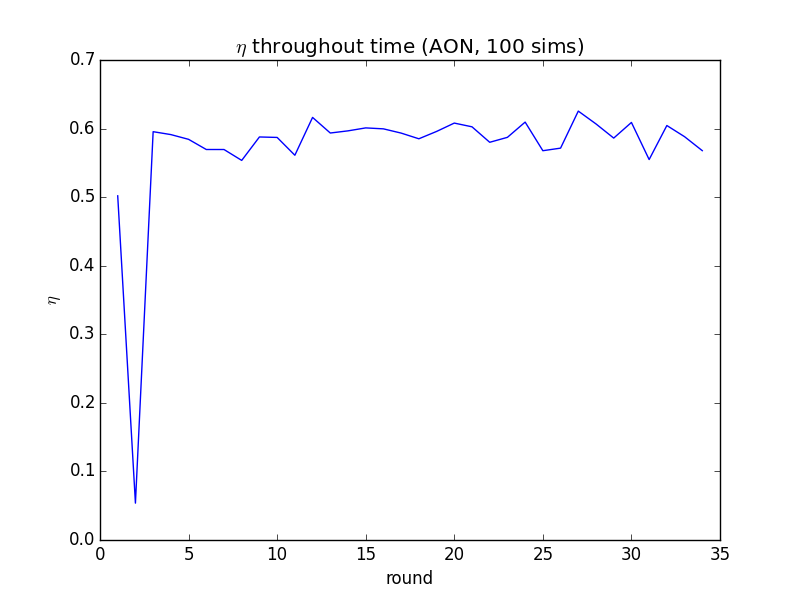
\includegraphics[width=3.6in,angle=0]{img/cfraction_aon.png}
\captionof{figure}{Cooperation fraction throughout time (100 sims). Where $Z=100$, $N=10$, $F=10$, $c= 2$, $\beta=1$, $\epsilon=0.05$, $\mu=0.01$ and the initial amount of \textbf{$C$} $= 0.5$}
\label{fig1}
As can be seen in Fig.~\ref{fig1} in the first round almost all simulations will go near 0.05. This is due to the fact that in the first round all choices are generated randomly. After this we get an average of 0.6 because of choice changes as a result of the $\epsilon$  value.
In Fig.~\ref{fig2} we will test the robustness of the \textbf{AON} strategy. As can be seen when $\epsilon$ is very low we get a high behavioral fraction as opposed to a high $\epsilon$. This result is to be expected, as an $\epsilon$ nearing zero stands for a group of AON players that almost never behave unexpectedly and will converge towards cooperating nearly every time.


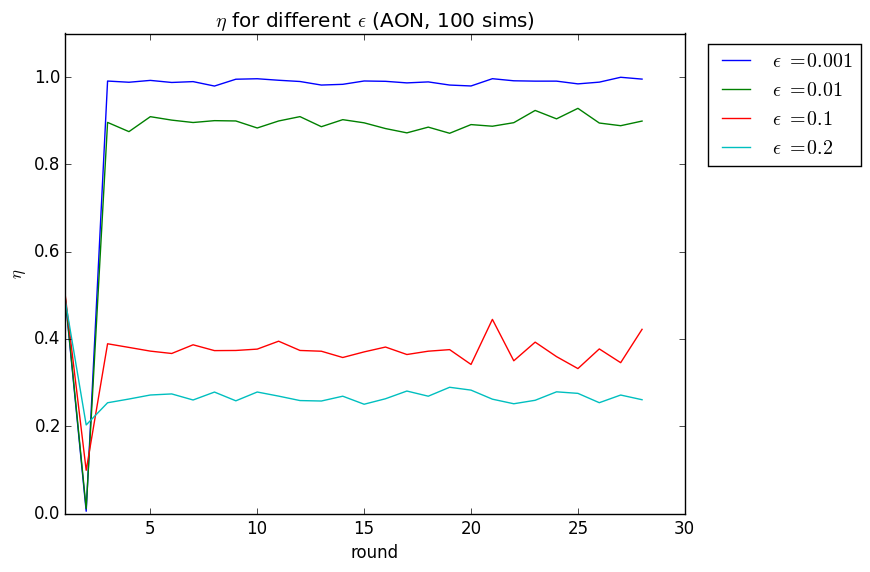
\includegraphics[width=3.6in,angle=0]{img/cfraction_epsilon_aon.png}
\captionof{figure}{Cooperation fraction throughout time (100 sims) with different $\epsilon$.}
\label{fig2}


% In Fig.~\ref{fig2}


As can be seen on Fig.~\ref{fig4} the higher the enhancement factor $F$ is, the higher the mean will be, which is a logical consequence. It is also shown that in these simulations, the strategy has a negative return if $F<2$.
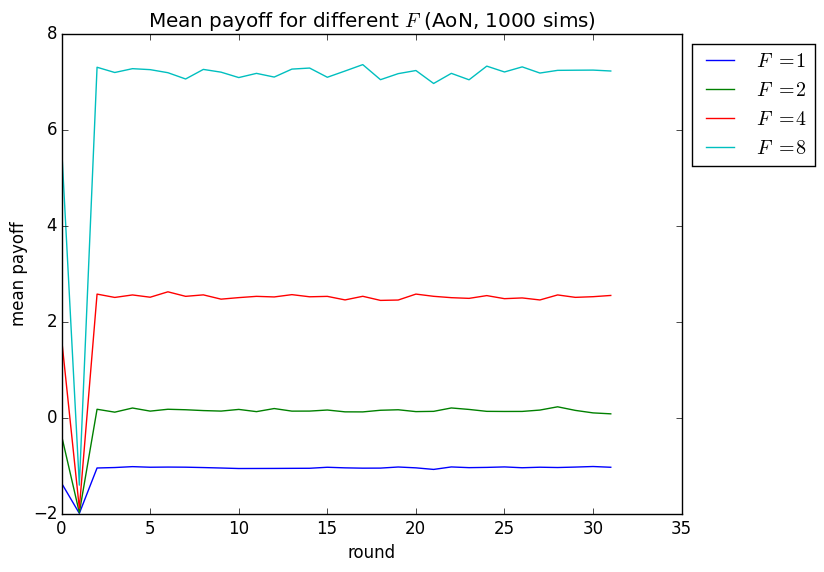
\includegraphics[width=3.6in,angle=0]{img/meanpayoff_F_aon.png}
\captionof{figure}{Mean payoff for different $F$}
\label{fig3}
Fig.~\ref{fig4} shows that there is not meaningful difference for different values of $F$. This is an intuitive result, seeing as none of the players using the AON strategy make use of the previous or expected payoff to choose C or D.
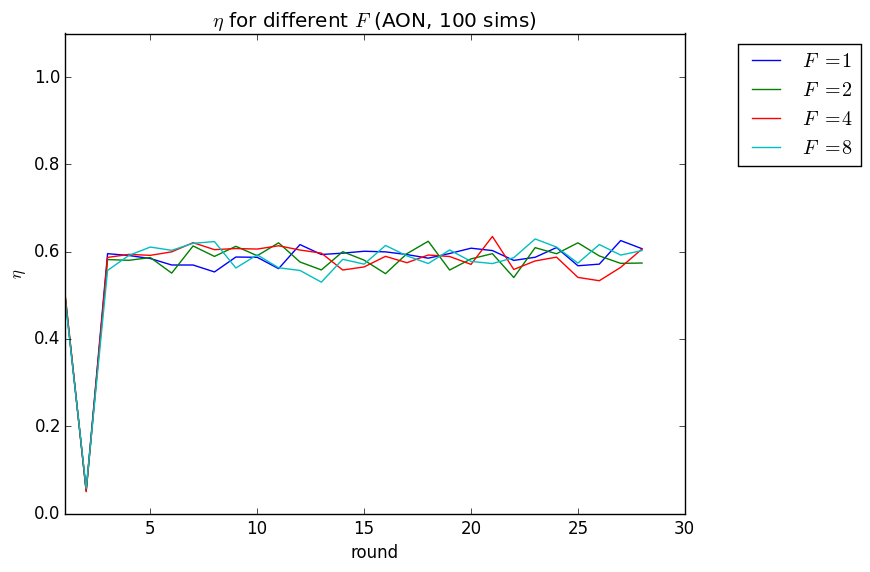
\includegraphics[width=3.6in,angle=0]{img/cfraction_F_aon.png}
\captionof{figure}{$\eta$ for different enhancement factor $F$}
\label{fig4}

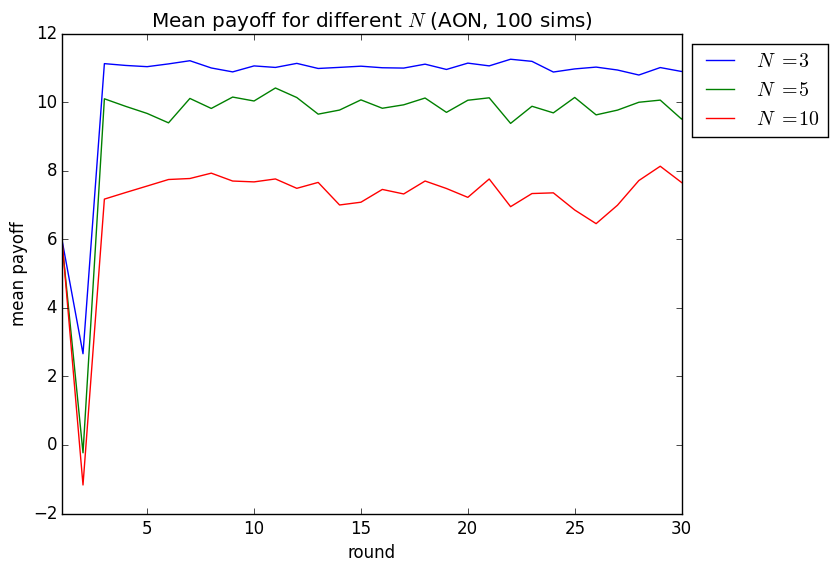
\includegraphics[width=3.6in,angle=0]{img/meanpayoff_N_aon.png}
\captionof{figure}{Mean payoff for different $N$}
\label{fig5}


AAIC = unconditional cooperators
\includegraphics[width=3.6in,angle=0]{img/cfraction_AONAllCfractions_aon.png}
\captionof{figure}{$\eta$ for different AON/AIIC}
\label{fig6}
AAID = unconditional defectors
\includegraphics[width=3.6in,angle=0]{img/cfraction_AONAllDfractions_aon.png}
\captionof{figure}{$\eta$ for different AON/AIID} 
\label{fig7}


\includegraphics[width=3.6in,angle=0]{img/meanpayoff_AONAllCfractions_aon.png}
\captionof{figure}{Mean payoff for different AON/AIIC}
\label{fig8}

\includegraphics[width=3.6in,angle=0]{img/meanpayoff_AONAllDfractions_aon.png}
\captionof{figure}{Mean payoff for different AON/AIID}
\label{fig9}

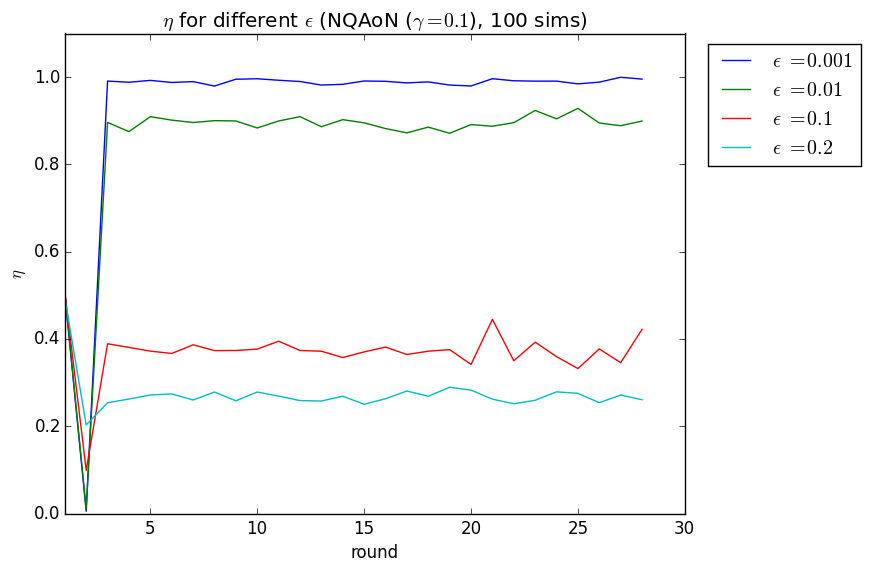
\includegraphics[width=3.6in,angle=0]{img/cfraction_epsilon_nqaongamma01.png}
\captionof{figure} {$\eta$ with $\epsilon$ $\gamma=0.01$}
\label{fig10}

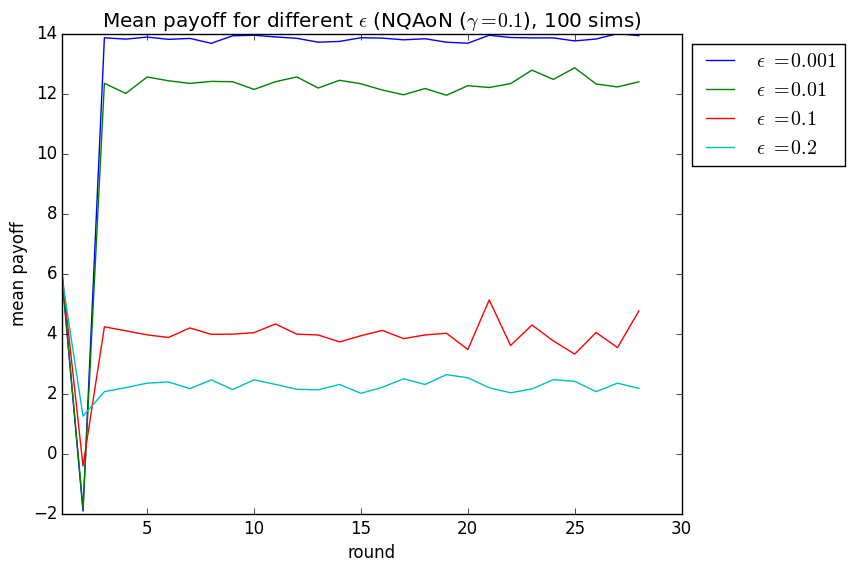
\includegraphics[width=3.6in,angle=0]{img/meanpayoff_epsilon_nqaongamma01.png}
\captionof{figure} {mean payoff with $\epsilon$ $\gamma=0.01$}
\label{fig11}

\section{Discussion}
Something something

\section{Acknowledgments}
github page

\footnotesize

\bibliographystyle{apalike}
\bibliography{biblio}


\end{document}
